%%7 делится на две главы. Задача с чертежом коорд.оси (предвор сведения, разработанные библ функции, шаблоны)
\section{Задачи №7 ОГЭ (координатная прямая)}

\subsection{разработка функции}
Наиболее значимая часть работы — это разработка функций для визуализации координатной прямой и точек на ней. 
Была создана универсальная функция, позволяющая отображать засечки и подписи в разных режимах.

Одним из ключевых элементов реализации автоматической генерации заданий стала функция $coordAxis_drawMarkPoint$. Она предназначена для отрисовки различных типов меток на координатной оси и их подписей.

\subsection{Назначение функции}
Функция решает задачу визуализации точек и вспомогательных обозначений на оси,
что является неотъемлемой частью заданий ОГЭ и ЕГЭ по математике.
С помощью данной функции возможно изображать:
\begin{itemize}
    \item закрашенные точки (``dot''),
    \item выколотые точки (``emptyDot''),
    \item засечки (``line''),
    \item отсутствие метки (``nothing'').
\end{itemize}

\lstinputlisting[]{code/7/drawMarkPoint.js} 

\subsection{Интерфейс функции}
Функция имеет следующий набор параметров:
\begin{itemize}
    \item \texttt{ct}~--- графический контекст Canvas,
    \item \texttt{coord}~--- координата по оси X,
    \item \texttt{text}~--- подпись для метки,
    \item \texttt{markForm}~--- форма метки: \texttt{dot}, \texttt{emptyDot}, \texttt{line}, \texttt{nothing},
    \item \texttt{textPosition}~--- расположение подписи: под осью (\texttt{underAxis}), над осью (\texttt{overAxis}), на оси (\texttt{onAxis}),
    \item \texttt{options}~--- дополнительные параметры (шрифт, цвет текста, толщина линии, смещение).
\end{itemize}

\subsection{Алгоритм работы}
\begin{enumerate}
    \item Сохраняются текущие параметры отрисовки (\texttt{fillStyle}, \texttt{strokeStyle}, \texttt{font}, \texttt{lineWidth}).
    \item Устанавливаются новые параметры, переданные в \texttt{options}.
    \item В зависимости от параметра \texttt{markForm} рисуется выбранный элемент:
    \begin{itemize}
        \item точка~--- закрашенный круг,
        \item выколотая точка~--- окружность с заливкой белым цветом внутри,
        \item засечка~--- вертикальная черта,
        \item отсутствие~--- элемент не отрисовывается.
    \end{itemize}
    \item В зависимости от параметра \texttt{textPosition} подпись размещается под осью, над осью или на линии оси.
    \item Восстанавливаются исходные параметры графического контекста.
\end{enumerate}

 \texttt{coordAxis\_prepare}, что позволяет подготовить область для оси и рисует стрелку. И
\texttt{coordAxis\_drawAuto} она автоматически вычисляет масштаб оси и вызывает $coordAxis_drawMarkPoint$ для всех точек.


Функция \texttt{coordAxis\_prepare} выполняет подготовку холста для отрисовки горизонтальной координатной оси со стрелкой.
Она:
\begin{itemize}
  \item задаёт габариты рабочей области оси (\verb|width|, \verb|height|) и сохраняет их в контексте для последующего использования;
  \item вертикально центрирует ось (Ox) (смещение системы координат);
  \item настраивает стили (цвет линии и толщину) и рисует ось со стрелкой;
  \item бережно восстанавливает исходные графические параметры контекста.
\end{itemize}
Компонент рассчитан на дальнейшее использование вместе с $coordAxis_drawMarkPoint$ и $coordAxis_drawAuto$.

\lstinputlisting[]{code/7/prepare.js} 

\begin{description}
  \item[\texttt{ct}] графический контекст \verb|CanvasRenderingContext2D|.
  \item[\texttt{width}] ширина области оси в пикселях, по умолчанию (400).
  \item[\texttt{height}] высота области в пикселях, по умолчанию (100).
  \item[\texttt{strokeStyle}] цвет линии оси (интеграция со стилем проекта через \verb|om.primaryBrandColors[0]|).
  \item[\texttt{lineWidth}] толщина линии оси, по умолчанию (2).
\end{description}

Функция явно сохраняет текущие значения \verb|strokeStyle| и \verb|lineWidth| в локальные переменные
\verb|prevStroke| и \verb|prevLineWidth| и восстанавливает их к концу выполнения.  
Параметры \verb|ct.__coordAxisW| и \verb|ct.__coordAxisH| записываются в контекст как служебные метаданные — это упрощает доступ к габаритам при последующих рисованиях (например, при авторазметке меток).

Важно, что вызывается \verb|ct.translate(0, height/2)|: система координат сдвигается на половину высоты вниз, чтобы ось (Ox) оказалась по центру холста. Этот сдвиг является \emph{накопительным}; поэтому рекомендуется либо:
\begin{itemize}
  \item вызывать \verb|coordAxis_prepare| один раз в рамках одного цикла отрисовки, либо
  \item оборачивать работу в \verb|ct.save() ... ct.restore()|, если требуется многократная подготовка в одном контексте.
\end{itemize}

\verb|coordAxis_prepare| задаёт «сцену» — габариты, позицию оси и её визуальные атрибуты. Поверх этой сцены функции \verb|coordAxis_drawMarkPoint| и \verb|coordAxis_drawAuto| размещают метки и подписи.
 Такое разделение обязанностей упрощает поддержку кода: изменения оформления оси не затрагивают логику генерации и размещения меток.
Данная функция является частью связки:
    
Из особенностей можно подчеркнуть что функция поддерживает как закрашенные, так и выколотые точки, что позволяет формировать задания с открытыми и закрытыми интервалами.
Так же она восстанавливает исходные параметры, гарантирует корректную работу при множественной отрисовке. А так же есть возможность смещения текста по оси X , что помогает избежать наложений подписей.
\lstinputlisting[]{code/7/drawAuto.js} 


\subsection{Пример использования}
\begin{verbatim}
// Отрисовка закрашенной точки A с подписью под осью
coordAxis_drawMarkPoint(ct, 100, "A", "dot", "underAxis");

// Отрисовка выколотой точки B с подписью над осью
coordAxis_drawMarkPoint(ct, 200, "B", "emptyDot", "overAxis");
\end{verbatim}

Пример работы:
\lstinputlisting[]{code/7/314802.js} 
До:
После:
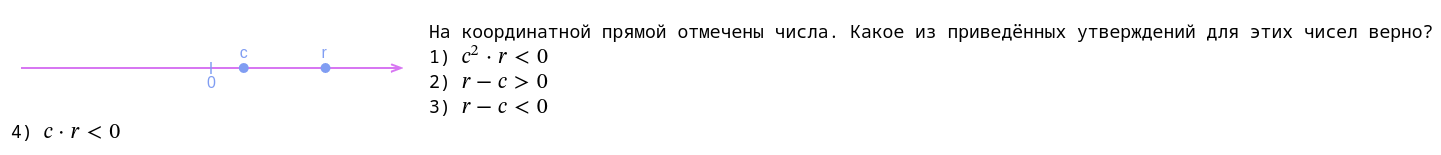
\includegraphics[width=0.4\textwidth]{314802-7-3.png}
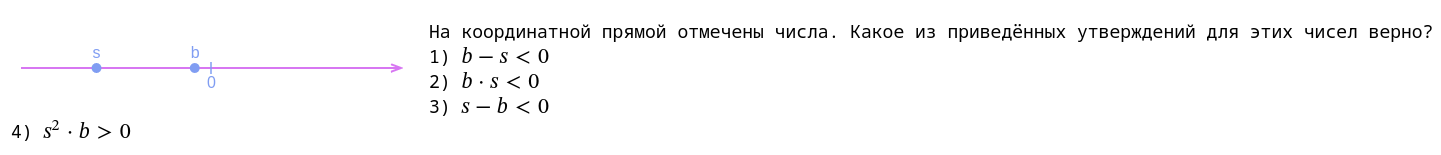
\includegraphics[width=0.4\textwidth]{314802-7-2.png}
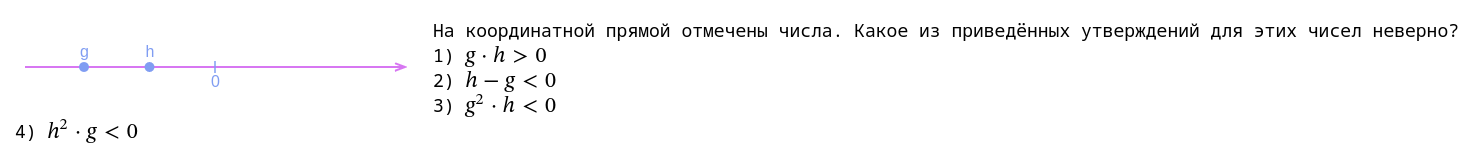
\includegraphics[width=0.4\textwidth]{314802-7-1.png}

\lstinputlisting[]{code/7/337301.js} 
До:
После:
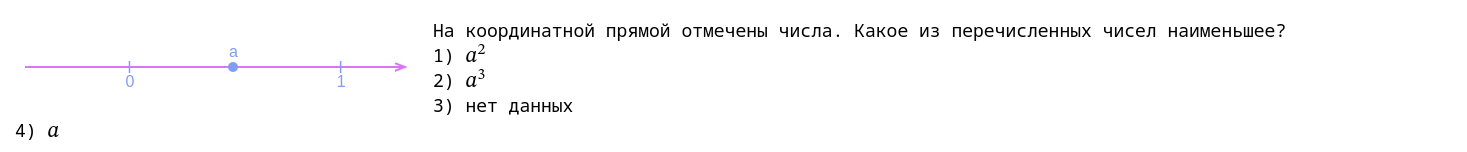
\includegraphics[width=0.4\textwidth]{337301-7-1.png}
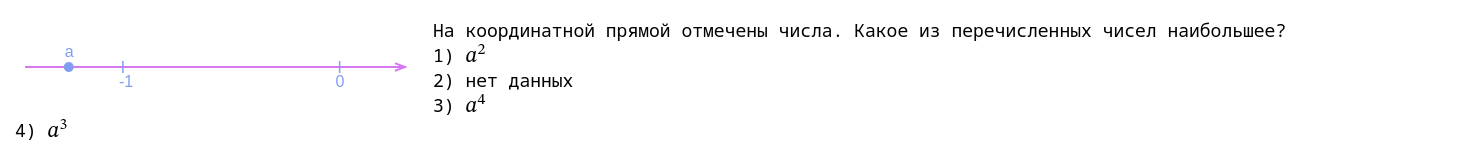
\includegraphics[width=0.4\textwidth]{337301-7-2.png}